\documentclass[addpoints,answers]{exam}
\usepackage{times}
\usepackage{epsfig}
\usepackage{listings}
\lstset{
basicstyle=\small\ttfamily,
columns=flexible,
breaklines=true
}

\lhead{\ifcontinuation{Question \ContinuedQuestion\ continues\ldots}{}}
\chead{ECE 422 / CS 461, Final Exam}
\rhead{Wednesday, May 6th, 2015}
\lfoot{Points: \makebox[.5in]{\hrulefill} / \pointsonpage{\thepage}}
\cfoot{\thepage\ of \numpages}
\rfoot{NetID:\enspace\makebox[1.5in]{\hrulefill}}

\qformat{\thequestiontitle\dotfill \emph{\totalpoints\ points}}

\begin{document}

\begin{titlepage}
  \vspace*{\fill}
  \begin{center}
    \Large\textbf{ECE 422 / CS 461, Final Exam}\\
    \large\textit{Wednesday, May 6th, 2015}\\
  \end{center}
  \vspace{.5in}
  \par\large{Name:}\hrulefill\\
  \par\large{NetID:}\hrulefill\\
  \vspace{.5in}
  \begin{itemize}
  \item Be sure that your exam booklet has \numpages\ pages.
  \item Write your net ID at the top of each page.
  \item Absolutely no interaction between students is allowed.
  \item Show all of your work.
  \end{itemize}
  \vspace*{\fill}
\end{titlepage}
\newpage 

\begin{center}
  \vspace*{\stretch{1}}
  \gradetable[v][pages]
  \vspace*{\stretch{1}}
\end{center}
\newpage

\begin{questions}

\titledquestion{Question \thequestion: Multiple Choice}

\textbf{For each question, circle all that apply.}

\begin{parts}

\part[1]

Sending a message in the presence of an eavesdropper without revealing
the message itself is ensuring which aspect of security?

\begin{choices}
\correctchoice Confidentiality
\choice Integrity
\choice Availability
\choice Authenticity
\end{choices}

\part[1]

A security breach that is caused or facilitated by someone who is a
part of the very organization that controls or builds the asset that
should be protected is which of the following?

\begin{choices}
\choice Backdoor
\correctchoice Insider Attack
\choice Logic bomb
\choice Trojan
\end{choices}

\part[1]

SSL/TLS protects which layer of the Internet?

\begin{choices}
\choice Physical
\choice Data Link
\choice Network
\correctchoice Transport
\end{choices}

\part[1]

Which one of the following C library functions is unsafe because it
has no parameter for the size of the input buffer that it will fill?

\begin{choices}
\choice snprintf
\choice fgets
\correctchoice gets
\choice strncpy
\end{choices}

\part[1]

Since there are 10000 possibilities for a 4 digit PIN, in the real
world, 4321 is the PIN for about 0.01\% of people's debit cards.

\begin{choices}
\choice TRUE
\correctchoice FALSE
\end{choices}

\pagebreak

\part[2]

Consider the following C++ code.  Assume the code compiles and runs,
that no operations were optimized out by the compiler, and that it
always receives one argument when called.

\begin{lstlisting}    
    #include <stdio.h>

    void derp(char* str)
    {
        char buff[256];
        strcpy(buff /*dest*/, str /*src*/);
    }
    
    int main(int argc, char** argv)
    {
        derp(argv[1]);
        printf("Hello World\n");
        return 0;
    }
\end{lstlisting}
    
Which of the following can NOT be achieved solely by manipulating the
parameter passed to this program when it is called (i.e., manipulating
the string pointed to by argv[1])?

\begin{choices}    
\choice Overwriting the return address of main()
\choice Changing what text is displayed by printf()
\correctchoice Overwriting executable instructions within derp()
\choice Overwriting the argc variable
\choice All of the following are possible
\end{choices}
    
\part[1]
    
You have 4 data blocks named A, B, C, and D of exactly 1KB each (assume no padding is added to any blocks when generating MD5 hashes):
\begin{lstlisting}
        - A, B, C, and D all contain different data
        - A and B have the same MD5 hash
        - C and D have the same MD5 hash
        - A and B's hash is different than C and D's hash
\end{lstlisting}    
    If we concatenate blocks A and C together to form the 2KB block AC, it will have the same MD5 hash as the 2KB block BD.
    
\begin{choices}
\correctchoice TRUE
\choice FALSE
\end{choices}

\part[1] 

What is the term used to describe the malicious action that a virus is supposed to perform?

\begin{choices}
\choice Trojan
\correctchoice Payload
\choice Backdoor
\choice Botnet
\end{choices}

\part[1] 

An attacker places the address of a series of gadgets on the
stack. What is she doing?

\begin{choices}
\correctchoice Return oriented programming
\choice Smashing the stack
\choice Conducting a formatted string attack
\choice None of the other answers are correct
\end{choices}

\pagebreak

\part[1] 

A token is an example of an authentication method based on what a user:

\begin{choices}
\choice is
\choice does
\choice knows
\correctchoice has
\end{choices}

\part[1]

Which of the following weaknesses did the Heartbleed bug exploit?

\begin{choices}
\correctchoice unchecked client inputs
\choice buffer overflows
\choice denial of service
\choice incorrect cross-domain origin settings
\end{choices}

\part[1]

A group of students managed to hack into their professor's computer
and obtained a copy of the final exam. As security measures, they all
encrypted their hard drives, disabled sleep mode and hibernation, and
used throw-away Gmail accounts for communication. A few days later,
one of them gets arrested at his apartment; unfortunately, he fails to
close the Internet browser or shut down the computer in time. Which of
the following evidence should be captured first?

\begin{choices}
\choice Internet browsing histories
\choice Hibernation files
\choice Deleted files
\correctchoice RAM data
\choice Removable media (USB drives, CD, etc.), if there is any
\end{choices}

\part[1]

In question 1(l), if the investigator determines that there are enough evidence without
hidden and residual data (e.g., slack space, swap, residue, unused
space, deleted files etc.), he may choose to do regular backups,
instead of bitstream.

\begin{choices}
\choice TRUE
\correctchoice FALSE
\end{choices}

\part[3]

Assume that you want to securely communicate with illinois.edu from
your home using TLS. Which of the following items will you need to
trust to be able to preserve confidentiality, integrity, and
authenticity when using TLS? 

\begin{choices}
\choice The entire network between you and illinois.edu
\choice Computers on your local, home network
\choice The operators of .edu's Authoritative DNS servers
\choice The operators of illinois.edu
\correctchoice illinois.edu's Certificate Authority (CA)
\choice All the CA's configured into illinois.edu's software
\correctchoice All the CA's configured into your browser
\correctchoice The designers of the cryptographic algorithms
\end{choices}

\end{parts}

\pagebreak

\titledquestion{Question \thequestion: Short Answer}

\begin{parts}

\part[2] 
Here are some evidence the investigator found from the student's computer
in question 1(l).

\begin{lstlisting}
auth.log
|...
|Apr 30 14:33:05 l337-h4x0r sudo:    h4x0r : TTY=pts/1 ; PWD=/home/h4x0r/ ; USER=root ; COMMAND=/usr/sbin/arpspoof 192.168.6.36 -t 192.168.6.61
|Apr 30 14:33:10 l337-h4x0r sudo:    h4x0r : TTY=pts/15 ; PWD=/home/h4x0r/ ; USER=root ; COMMAND=/usr/sbin/arpspoof 192.168.6.61 -t 192.168.6.36
.bash_history
|...
|nmap -A 192.168.6.0/24
known_hosts
|192.168.10.58
|192.168.6.36
|192.168.6.41
|192.168.6.51
|192.168.6.61
syslog
|...
|Apr 30 14:05:15 l337-h4x0r NetworkManager[1065]: <info> (eth0): DHCPv4 state changed renew -> renew
|Apr 30 14:05:15 l337-h4x0r NetworkManager[1065]: <info>   address 192.168.6.37
|Apr 30 14:05:15 l337-h4x0r NetworkManager[1065]: <info>   prefix 24 (255.255.255.0)
|Apr 30 14:05:15 l337-h4x0r NetworkManager[1065]: <info>   gateway 192.168.6.61
|Apr 30 14:05:15 l337-h4x0r NetworkManager[1065]: <info>   nameserver '192.168.6.61'
\end{lstlisting}

Identify the professor's (the victim's) IP address.

\begin{solutionorbox}[1in]
192.168.6.36
\end{solutionorbox}

\part[2]

Why do shellcoders usually put effort into avoiding zero (NULL)
characters/bytes in their shellcode?

\begin{solutionorbox}[1in]    
strcpy stops at '\textbackslash 0'
\end{solutionorbox}

\part[2]

Name two countermeasures against buffer overflow attacks.

\begin{solutionorbox}[1in]    
\begin{lstlisting}
(1) Address Space Layout Randomization
(2) Disabling execution of instructions on the stack
(3) Restricting the number of bytes copied during copy operations
\end{lstlisting}
\end{solutionorbox}

\pagebreak

\part[2]

Consider the following message protocol for establishing group
membership with secret k:

\begin{lstlisting}
User A sends random nonce n1 to User B
User B sends back Hash_k(n1) and random nonce n2
User A verifies Hash_k(n1) then sends back Hash_k(n1 | n2) 
User B verifies and group membership is established.
\end{lstlisting}

Is this protocol safe? Explain.

\begin{solutionorbox}[1in]   
This protocol still gives up too much information before the conversation initiator has proved its knowledge of the key. By beginning a conversation with B with nonce n1, C can receive the n2 nonce from B and send nonce (n1 | n2) to A to initiate conversation, take the hash A sends back and confirm group membership with B. 
\end{solutionorbox}

\part[2]

Give two examples of password hashing strategies to defend against rainbow table attacks.

\begin{solutionorbox}[1in] 
1.) salted hashes, 2.) slower hash functions   
\end{solutionorbox}

\end{parts}

\pagebreak

\titledquestion{Question \thequestion: Spoofing}
Suppose some networks and the Internet are configured as described and shown
below and do not use firewalls or filtering:

\begin{figure}[h!]
  \centering
    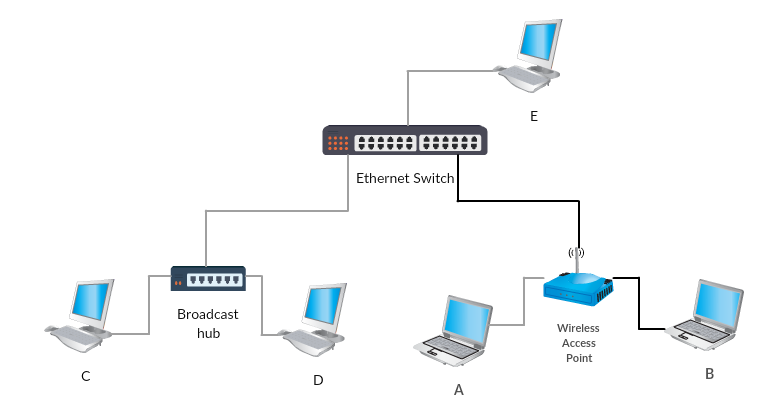
\includegraphics[width=0.7\textwidth]{net}
      \caption{Question 3}
\end{figure}

\begin{itemize}
\item Hosts A and B are laptops on ECE 422, which is an open WiFi network on campus, subnet: 192.168.150.0/25.
\item Host C is a wired desktop connected to Illinois' networks, subnet: 192.168.150.128/25.
\item R is the edge router of Illinois' network, subnet: 192.168.140.0/24.
\item D is a laptop running on a different autonomous system (AS) auton1.
\item E is a laptop running on a different AS auton2.
\end{itemize}

\begin{parts}

\part[2] 

Suppose that there is a TCP session between A and B. How can an
attacker who has access to ECE 422 and knows A and B's IP addresses
eavesdrop that TCP session without interrupting it? Explain the steps
the attacker needs to take and specify what each step achieves.

\begin{solutionorbox}[1in]    
Solution 1 (active): 2 steps of arpspoof plus one step of IP forwarding, each +1 point. +1 point for correct ordering; i.e., IP forwarding first.
Solution 2 (passive): eavesdrop traffic with tools such as wireshark (preconscious or monitor modes) or other capturing tools.
\end{solutionorbox}

\part[3] 

Suppose that an attacker wants to initiate and complete a TCP
handshake with a victim, such that the victim thinks that E initiated
the connection. Assume that TCP uses a modern implementation, the
attack is restricted to use no more than a half dozen packets, and
that the attacker knows the victim's and E's IP addresses. Answer
the following three questions.

\begin{lstlisting}
Among B, C, D, and R which ones can attack A (i.e., victim=A)? Why?
Among A, B, D, and R which ones can attack C (i.e., victim=C)? Why?
Among A, B, C, and R which ones can attack D (i.e., victim=D)? Why?
\end{lstlisting}

\begin{solutionorbox}[1in]    
B and R can attack A; R can attack C and none of them can attack D.

TCP's Initial Sequence Numbers (ISNs) will be randomized. So, the
attacker needs to either eavesdrop on traffic sent from the victim or
it should be in the forwarding path between the victim and E for the
attack to work with a half dozen packets.

each correct answer: +1, each wrong answer: -1, each correct reasoning: +1 (overall grade $>=0$)
\end{solutionorbox}

\end{parts}

\pagebreak

\titledquestion{Question \thequestion: Port Scan}

\begin{parts}

\part[3]

What are the goals of a port scan attack? Circle all that
apply.

\begin{choices}
\correctchoice Identifying active services
\choice Discovering usernames and passwords
\choice Disabling active ports
\correctchoice Identifying operating systems
\correctchoice Identifying potential vulnerabilities
\choice Poisoning ARP caches
\end{choices}

\part[2]

Assume that an attacker has joined a protected WiFi network. Suggest a
way for the attacker to carry out a port scan against the hosts on the
same network in order to achieve one of the above goals. Suggest the
tool(s) that the attacker needs to use and the steps to carry out the
attack.

\begin{solutionorbox}[1in]
nmap. with different parameters for different goals. other
tools/solutions could be acceptable. correct tool: +1. correct steps:
+1
\end{solutionorbox}


\part[2]

How can the operator of that WiFi network detect that attack?

\begin{solutionorbox}[1in]
different tools that they know about for monitoring the network to
detect the suspicious activity, correct tool: +1. correct steps: +2
\end{solutionorbox}

\end{parts}

\pagebreak

\titledquestion{Question \thequestion: Cryptography}

\begin{parts}

\part

Alice and Bob are discussing their homework through an online
messenger. Eve, who is concerned about her curved grade, decides to
perform man-in-the-middle attack to alter the solution Alice was
sending to Bob. Alice and Bob did not yet learn about HMAC, so they
encrypt with a SHA-1 hash. SHA-1 takes multiple 512-bit blocks and
produces a 160-bit (20 bytes) hash value. They previously shared each
other's private keys offline for integrity purposes. The original
message is the concatenation of the sender's private key and the
solution to the homework, \texttt{message = (private\_key $\|$ solution)}.

\begin{subparts}

\subpart[2]

What information is/are needed for Eve to attack successfully?

\begin{solutionorbox}[1in]
[1 point] private key length
	[1 point] solution length
	OR [2 points] total length of the original message
\end{solutionorbox}	

\subpart[2]
	
Let's say Alice's private key is "crypto" (without quotation). Eve has
5 guesses on the correct solution: 1) chicken, 2) egg, 3) pig, 4) dog
and 5) penguin. Assuming that Eve has only 1 chance, what is the attack 
success rate?

\begin{solutionorbox}[1in]
50\%
\end{solutionorbox}	

\subpart[4]

Eve has chosen "penguin" to try the length-extension attack. She wants
to deceive Bob into believing that the solution is "bird" and tries to
append the message "no it is actually bird". What would the message
from Eve to Bob would look like? Describe the hash function as a
formula.

\begin{solutionorbox}[1in]
SHA\_1(crypto $\|$ penguin $\|$ padding((6+7)*8) $\|$ no it is actually bird)
\end{solutionorbox}	

\end{subparts}

\part[3]

Cathy is writing a report for her computer security course. At the end
of the report, she leaves a note to the professor but doesn't want to be
seen by her friends. So she decides to encrypt using a product cipher,
which is the combination of a substitution cipher and a transposition
cipher. The Vigenere cipher was used for substitution and then an
irregular columnar transposition cipher was applied to obtain the
final encrypted message. The encrypted message and keys for each
cipher are as below. Decrypt the message. Show your work for possible
partial credit.

\begin{lstlisting}
Encrypted message: "rgyqhbmnwaazxcajittuzqyagkx"
Vigenere cipher key: "final"
Columnar transposition cipher: "exam"
\end{lstlisting}

\begin{solutionorbox}[1in]
[2 points] Original plaintext: ``I really want an A for this course.''
	[1 point: partial] Encoded with Vigenere cipher: ``n zrawqg jayy ia a qtz ghtxkbucxm''
\end{solutionorbox}

\end{parts}

\pagebreak

\titledquestion{Question \thequestion: Forensics}

A murder happened on April 30th at approximately 6 PM in front of dunkin
donuts in Champaign. An hour later, police officers were able to obtain 
multiple hard disks on site. Those were sent out to the digital forensics 
department who found that all but two hard disks were wiped clean. Bob was 
recently hired in the digital forensics team and was given these as his 
first case to investigate. As he started to investigate, he was so excited 
and booted the hard disk on a machine, selected a disk partition, and 
started to explore. He navigated through the system's directories and 
opened a few log files to look for the evidence. Then, he realized 
something was wrong.

Fortunately, a more experienced expert, Cathy, duplicated the original
disk images before Bob started investigating. Through Autopsy, she
extracted few files on each of the two hard drives that might be
relevant to the case. These are listed on the following two pages.

\begin{parts}

\part[2]

What are the two main reasons that Bob made a big mistake? 

\begin{solutionorbox}[1in]
[1 point] tampering of the data: e.g. last modified time of the file 
gets changed, bash history gets overwritten
	[1 point] suspect may have pre-setup the partition to prevent from 
live analysis (obfuscate with other OS partition, disk wiping etc.)
(optional) attacking of the system is maybe needed to log on
\end{solutionorbox}

\part[2]

Who are the users of each of the hard disks?

\begin{solutionorbox}[1in]
[1 point] Hard disk 1: naive
	[1 point] Hard disk 2: innocent
\end{solutionorbox}

\part[3]

What were the main activities of two users for each hard disk? 
Explain in time order for each hard disk.

\begin{solutionorbox}[1in]
[1.5 points] Naive (130.126.136.203): Email logged in. Searched and read email from innocent. (Email account left logged on) <possibly got murdered> Account was remotely logged on (using Hydra). Bash history got deleted. Internet browser got opened. Email was searched with from:innocent@gmail.com. Email was removed to trash. Email account logged out. Shut down.
	[1.5 points] Innocent (130.126.136.200): Email logged in. Composed email to naive@gmail.com. Deleted sent email. Email logged out. <possibly murdered the victim> Hacked into naive's machine remotely. (on remote machine) Activity on Naive's log. Disconnected remote connection. Shut down.
\end{solutionorbox}

\part[3]

Are the evidences you found from (c) relevant to this case? If so, who 
do you think is the criminal? The owner of the first hard disk, the second,
or both?

\begin{solutionorbox}[1in]
Second. Naive is the victim. Innocent contacted the victim via email
to lure into a trap, hacked the victim's machine to delete the
email history.
\end{solutionorbox}

\end{parts}

\pagebreak
THIS PAGE IS INTENTIONALLY LEFT BLANK
\pagebreak

\begin{lstlisting}
<Hard Disk 1>
Directory: /var/log/
1) auth.log
|...
|Apr 30 17:02:30 naive login: session opened for user naive by LOGIN(uid=0)
|Apr 30 17:02:32 naive login: NAIVE LOGIN ON 'tty1'
|...
|Apr 30 18:01:20 naive sshd: server listening on :: port 22
|Apr 30 18:23:00 naive sshd: Invalid user innocent from 130.126.136.200
|Apr 30 18:23:03 naive sshd: Failed none for invalid user innocent from 130.126.136.200
|Apr 30 18:23:20 naive sshd: authentication failure; rhost=130.126.136.200, ruser=naive
|Apr 30 18:23:47 naive sshd: Failed password for naive from 130.126.136.200 server listening on :: port 22
|... repeated password failures
|Apr 30 18:50:29 naive sshd: Accepted password for naive from 130.126.136.200 server listening on :: port 22
|...
|Apr 30 18:53:05 naive sshd: server listening on :: port 22

Directory: /home/naive/
1) .ssh/known_hosts
|99.118.111.49
|141.212.111.41

2) .bash_history
|...
|cat .bash_history
|rm .bash_history
|firefox &
|shutdown -h now
|exit

3) Hydra log
|...
|130.126.136.203
|hydra


4) .mozilla/firefox/places.sqlite
|...
|https://mail.google.com/
|https://mail.google.com/mail/u/0/#inboxInbox (54) - naive@gmail.com - Gmail...
|https://mail.google.com/mail/u/0/#search/innocent
|https://mail.google.com/mail/u/0/#inbox/14d281606fc2d482...
|...
|https://www.google.com/maps/search/@40.114719,-88.2442045,13zdunkin+donuts+near+me - Google Maps...
|...
|https://mail.google.com/mail/u/0/#inboxInbox (53) - naive@gmail.com - Gmail...
|https://mail.google.com/mail/u/0/#search/from%3A+innocent%40gmail.com/14d2816b7a04c3ffURGENT! Please come to dunkin donuts at 5:50pm - naive@gmail.com - Gmail...
|https://mail.google.com/mail/u/0/#inbox/14d2816b7a04c3ff
|https://mail.google.com/mail/u/0/#trashTrash - naive@gmail.com - Gmail
\end{lstlisting}

\pagebreak
THIS PAGE IS INTENTIONALLY LEFT BLANK
\pagebreak

\begin{lstlisting}
<Hard Disk 2>
Directory: /var/log/
1) auth.log
|...
|Apr 30 16:48:23 innocent-laptop CRON: session opened for user innocent by (uid=0)
|Apr 30 16:48:53 innocent-laptop CRON: session opened for user root by (uid=0)
|Apr 30 16:51:00 innocent-laptop CRON: session closed for user root by (uid=0)
|Apr 30 16:52:30 innocent-laptop gdm: authentication failure user=innocent
|...
|Apr 30 18:00:02 innocent-laptop gdm: session opened for user innocent by (uid=0)
|Apr 30 18:05:02 innocent-laptop sudo: /home/innocent/hydra-5.4-src ; USER=root ; COMMAND = /usr/bin/aptitude install libssh-2
|Apr 30 18:05:14 innocent-laptop sudo: /home/innocent/hydra-5.4-src ; USER=root ; COMMAND = /usr/bin/aptitude install libssh-2-dev
|Apr 30 18:05:59 innocent-laptop sudo: /home/innocent/hydra-5.4-src ; USER=root ; COMMAND = /usr/bin/aptitude install libssh-2
|...
|Apr 30 18:22:30 innocent-laptop sudo: innocent: TTY=pts/0 ; PWD=/home/innocent/hydra-5.4-src ; USER=root ; COMMAND=/sbin/ifconfig eth0 130.126.136.200
|Apr 30 18:22:59 innocent-laptop gdm: session opened for user innocent by (uid=0)
|Apr 30 18:23:03 innocent-laptop CRON: session closed for user innocent by (uid=0)
|Apr 30 18:24:32 innocent-laptop gdm: session opened for user naive by (uid=0)
|Apr 30 18:25:01 innocent-laptop CRON: session closed for user naive by (uid=0)
|... repeat
|Apr 30 18:50:29 innocent-laptop gdm: session opened for user naive by (uid=0)
|Apr 30 18:53:05 innocent-laptop CRON: session closed for user naive by (uid=0)
|Apr 30 18:53:07 innocent-laptop gdm: session closed for user innocent

Directory: /home/innocent/
1) .ssh/known_hosts
|99.118.111.49
|130.126.136.202
|130.126.136.203
|141.212.111.36
|141.212.111.41

2) .bash_history
|rm ~/.bash_history
|shutdown -s
|exit

3) Hydra log
|...
|130.126.136.200
|hydra

4) .mozilla/firefox/places.sqlite
|https://mail.google.com/mail/u/0/#inbox
|https://mail.google.com/mail/u/0/?pli=1#inbox?compose=new
|https://mail.google.com/mail/u/0/#inbox?compose=14d281634387aba5...
|...
|https://mail.google.com/mail/u/0/#sent?compose=14d2835246e93e12...
|https://mail.google.com/mail/u/0/#sentSent Mail - naive@gmail.com - Gmail...
|https://mail.google.com/mail/u/0/#trashTrash - tkdlezz@gmail.com - Gmail...
|https://mail.google.com/LogOut?service=mail&continue=https://mail.google.com/mail&hl=enGoogle Accounts...

\end{lstlisting}

\pagebreak

\titledquestion{Question \thequestion: Application Security}

Consider the following function:

\begin{lstlisting}
void foo(char *arg)
{
   ... 
   char buf[32];
   strcpy(buf, arg);
}
\end{lstlisting}

\textbf{arg} is a pointer to a char string that is the command line input from the user.  
Make these assumptions:
\begin{itemize}
\item The machine is a 32-bit little-endian system that behaves like the VM from MP4.
\item There are no defenses such as ASLR, stack canaries, or a non-executable stack (DEP)
\item You see the following information when the program is run in gdb and you set a breakpoint at foo with the command \texttt{break foo} :
\begin{itemize}
\item \textbf{buf} begins at 0xbffebfb0. 
\item $(gdb)$  x/2wx \$ebp\\
0xbffebfd8: 0xbffec068 0x08048fe1
\end{itemize}
\end{itemize}

\begin{parts}

\part[1]

Assuming there is no buffer overflow, what will be the value stored in \texttt{\$ebp} when \texttt{foo} returns?

\begin{solutionorbox}[1in]
0xbffec068 - all or nothing
\end{solutionorbox}


\part[1]

What is the memory address of the "return address" of the function that called \texttt{foo}?

\begin{solutionorbox}[1in]
0xbffec06c - all or nothing
\end{solutionorbox}

\pagebreak

\part[3]

You want to run a payload that is 24 bytes long and works like the shellcode
provided in MP4. Write the bytes that should be copied to the buffer for the most
concise possible exploit. Fill in one byte (in hex) per blank; use as many or few as you
need. Draw a box around the positions that will contain the payload and write shellcode.\\\\

\underline{\hspace{1.2cm}}\hspace{.2cm}
\underline{\hspace{1.2cm}}\hspace{.2cm}
\underline{\hspace{1.2cm}}\hspace{.2cm}
\underline{\hspace{1.2cm}}\hspace{.2cm}
\underline{\hspace{1.2cm}}\hspace{.2cm}
\underline{\hspace{1.2cm}}\hspace{.2cm}
\underline{\hspace{1.2cm}}\hspace{.2cm}
\underline{\hspace{1.2cm}}\\\\
\underline{\hspace{1.2cm}}\hspace{.2cm}
\underline{\hspace{1.2cm}}\hspace{.2cm}
\underline{\hspace{1.2cm}}\hspace{.2cm}
\underline{\hspace{1.2cm}}\hspace{.2cm}
\underline{\hspace{1.2cm}}\hspace{.2cm}
\underline{\hspace{1.2cm}}\hspace{.2cm}
\underline{\hspace{1.2cm}}\hspace{.2cm}
\underline{\hspace{1.2cm}}\\\\
\underline{\hspace{1.2cm}}\hspace{.2cm}
\underline{\hspace{1.2cm}}\hspace{.2cm}
\underline{\hspace{1.2cm}}\hspace{.2cm}
\underline{\hspace{1.2cm}}\hspace{.2cm}
\underline{\hspace{1.2cm}}\hspace{.2cm}
\underline{\hspace{1.2cm}}\hspace{.2cm}
\underline{\hspace{1.2cm}}\hspace{.2cm}
\underline{\hspace{1.2cm}}\\\\
\underline{\hspace{1.2cm}}\hspace{.2cm}
\underline{\hspace{1.2cm}}\hspace{.2cm}
\underline{\hspace{1.2cm}}\hspace{.2cm}
\underline{\hspace{1.2cm}}\hspace{.2cm}
\underline{\hspace{1.2cm}}\hspace{.2cm}
\underline{\hspace{1.2cm}}\hspace{.2cm}
\underline{\hspace{1.2cm}}\hspace{.2cm}
\underline{\hspace{1.2cm}}\\\\
\underline{\hspace{1.2cm}}\hspace{.2cm}
\underline{\hspace{1.2cm}}\hspace{.2cm}
\underline{\hspace{1.2cm}}\hspace{.2cm}
\underline{\hspace{1.2cm}}\hspace{.2cm}
\underline{\hspace{1.2cm}}\hspace{.2cm}
\underline{\hspace{1.2cm}}\hspace{.2cm}
\underline{\hspace{1.2cm}}\hspace{.2cm}
\underline{\hspace{1.2cm}}\\\\
\underline{\hspace{1.2cm}}\hspace{.2cm}
\underline{\hspace{1.2cm}}\hspace{.2cm}
\underline{\hspace{1.2cm}}\hspace{.2cm}
\underline{\hspace{1.2cm}}\hspace{.2cm}
\underline{\hspace{1.2cm}}\hspace{.2cm}
\underline{\hspace{1.2cm}}\hspace{.2cm}
\underline{\hspace{1.2cm}}\hspace{.2cm}
\underline{\hspace{1.2cm}}\\\\

\begin{solution}
shellcode follow by 20 bytes of ``A'' or similar character (not
'\textbackslash x00') follow by 0xbffebfb0.  Variation allows for other position of
shellcode as long as return address comes after 44 bytes and it points
to the shellcode or an nop sledge.Rubric: 1 point - return address is
in the correct place 1 point - return address is a correct value 1
point - payload is exactly 48 bytes long
\end{solution}

\part[4]

For this question, assume that ASLR is enabled, which results in the
stack being offset by 0-15 bytes each time it runs.  Assume that the
stack condition from the previous parts holds when the offset is 0.
Describe a payload in the form of a python print statement that will
\textbf{always} get the shellcode from part (c) to execute, or
explain why such a payload is impossible.  Try to make your payload as
concise as possible.  Assume that the shellcode is stored in a
variable named \texttt{shellcode}.

\begin{solutionorbox}[1in]
44 bytes of "garbage" or nops, then 0xbffebfef, then ``\textbackslash x90''*15, then shellcode.
The main point is for the student to understand that the shellcode
does not have to live in the buffer.

Rubric:
If the structure of the payload is correct:
+1 point for correct structure
+1 point return address in correct position 
+1 point correct value for return address (at least 0xbffebfef)
+1 point use nop sled of size at least 15 

If the student tries to put nop sled follow by shellcode in buffer then follow by a return address:
Case 1: works some of the time
+1 point if structure is nopsled + shellcode + return\_addr
+1 point for correct return address location
+1 point if return address's value is somewhere between 0xbffebfb0 and the beginning of shellcode

Case 2: correct nop sled length and return address's value but return address in the wrong location
+1 point if structure is nopsled + shellcode + return\_addr
+1 point if nop sled length is at least 15
+1 point if return address's value is at least 0xbffebfbf

If the student answers "No" with a reason that the buffer is not big enough, total is 1 point.

\end{solutionorbox}

\part[1]

For this question, assume that DEP is enabled.  Name a technique that an attacker could use to exploit this vulnerability in spite of DEP.

\begin{solutionorbox}[1in]
return to libc or return oriented programming - all or nothing
\end{solutionorbox}

\end{parts}

\newpage

\titledquestion{Question \thequestion: SQL Injection}

Suppose we have a php web server that stores users' information in a
SQL database to implement an authentication system.  The website has a
login page with username and password fields, which are submitted to
the server in a POST request.  The following code snippet shows how
the php file interacts with the database.

\begin{lstlisting}
1 if (isset($_POST['username']) and isset($_POST['password'])) { 
2     $username = $_POST['username'];
3     $password = mysql_real_escape_string($_POST['password']);
4
5     $query = "SELECT * FROM users WHERE username='$username' and password='$password'";
6     $results = mysql_query($query);
7 }
\end{lstlisting}

Assume that the SQL server is the same as the SQL server used in MP2
and that the mysql\_real\_escape\_string() function fully sanitizes
the input by escaping all the special characters in the SQL language.

\begin{parts}

\part[2]

What is the input in the username field that will allow an attacker
to login as a user with username \texttt{victim}? Explain.

\begin{solutionorbox}[1in]
victim' ; --
Rubric:
+1 using OR [tautology]
+1 comment at the end
\end{solutionorbox}

\part[3]

Now, suppose that in an alternate implementation, the php server now
uses a sanitize function to replace all occurrence of ' with
$\backslash$' in the username and password string.  In other words,
lines 2 and 3 in the above implementation changes to:\\

\begin{lstlisting}
2     $username = sanitize($_POST['username']);
3     $password = sanitize($_POST['password']);
\end{lstlisting}

Assuming the input in the username field is \texttt{victim}, what
input in the password field will circumvent this defense and allows an
attacker to login as \texttt{victim}? Explain. \\

\begin{solutionorbox}[1in]
\' OR 1 = 1 ; --
Rubric:
+1 using tautology and comment at the end
+2 use \ to escape the backslash
\end{solutionorbox}

\end{parts}

\pagebreak

\titledquestion{Question \thequestion: CSRF and XSS}

JSONP is a communication technique used in Javascript programming to
circumvent the same-origin policy by executing a cross-domain GET
request through the script tag.  The protocol works by having the
caller execute a GET request by putting it in the src attribute of the
script tag and specifing a callback function.  For example: \\

\texttt{<script src="https://api.domain.com/status.json?callback=foo">}\\

Since a GET request through a script tag is not blocked by the
same-origin policy, the request will be sent to api.domain.com, who
will then process any input and send back data in the form of\\

\texttt{foo(data);}\\

Which will execute the caller-defined callback function foo with the data as its parameter on the caller's website.

\begin{parts}

\part[1] 

Suppose a website uses JSONP to make an API call to a malicious
server.  Describe how the malicious server could leverage this to
perform an XSS attack on the website.

\begin{solutionorbox}[1in]
the answer is JSONP is dangerous because the attacker can return any javascript and it will be execute in the user's browser. 1 point All or nothing
\end{solutionorbox}

\part[2]

Now, suppose that there is an online banking service that has a JSONP
API, and one of the API function calls available is
\\ \texttt{http://api.bank.com/getData?callback=[callback\_function\_name]},
which returns the user's data object for the logged-in user.  Assume
that the user is currently logged in to the bank's website and that the
attacker can trick the user into opening a website hosted on their
domain.  Describe a CSRF attack that allows the attacker to steal the
user's data and send it as a GET request to
``http://attacker.io/data=[\texttt{stolen\_data}]''.

\begin{solutionorbox}[1in]
The attacker's website contain a JSONP call to the bank's API, with
a callback function name foo.  The API call will return as
foo(user\_data).  Implement foo(user\_data) to send ajax request with
user's data to the attacker's url.  This attack is not possible
without JSONP because same-origin policy won't allow the attacker's
website to programmatically read the data +1 call the jsonp with
script tag +1 define callback function to forward the data 

\end{solutionorbox}

\part[2]

Is the attack from the last part possible if the bank's API does not support
JSONP (i.e., if the API call only returns the user's data without
invoking the callback)? Briefly explain why or why not.

\begin{solutionorbox}[1in]
The attack will not be possible becuase SOP would prevent the script from reading the response of the API call.
+1 Saying the attack is not possible without JSONP
+1 mentioning SOP in reason or mention that data cannot be read
\end{solutionorbox}

\end{parts}

\end{questions}

\end{document}
